\section{Introduction}

Statistics is concerned with scientific methods for collecting, organising, summarising, presenting and analysing data as well as deriving valid conclusions and making reasonable decisions on the basis of this analysis.

The major difference between machine learning and statistics is their purpose. \textit{Machine learning} models are designed to make the most accurate predictions possible. \textit{Statistical models} are designed for inference about the relationships between variables.

\subsection{Linear regression}

\textit{Linear regression} be regarded both as a statistical model and as a machine learning model:

\begin{itemize}
	\item \textbf{Statistical model}: it finds a line that minimizes the mean squared error over all data, having the primary goal to characterize the relationship between the data (covariates) and the output (dependent variable). The model is evaluated through error analysis, confidence instervals, significance tests, etc.
	\item \textbf{Machine learning}: a linear regression can be trained to achieve the best possible prediction. The training is performed on the \textit{training set}, to maximize the accuracy on the \textit{test set}. The model is evaluated based on the accuracy obtained on the test set.
\end{itemize}

\begin{figure}[H]
	\centering
	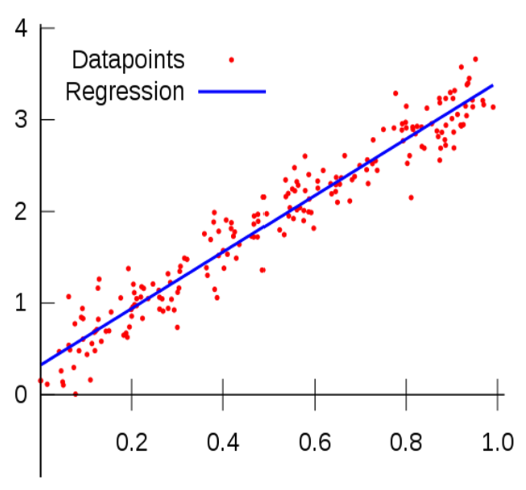
\includegraphics[width=0.4\textwidth]{images/linear-regression}
\end{figure}

\subsection{Multivariate data}

When analyzing complex systems, we work with multivaraite data, which can be represented as a matrix $\mathbb X = [x_{ij}] \in \mathbb R^{m \times n}$.

Consider the following example: \textit{quantity of products sold vs yearly marketing expenditures on each channel}.

\begin{figure}[H]
	\centering
	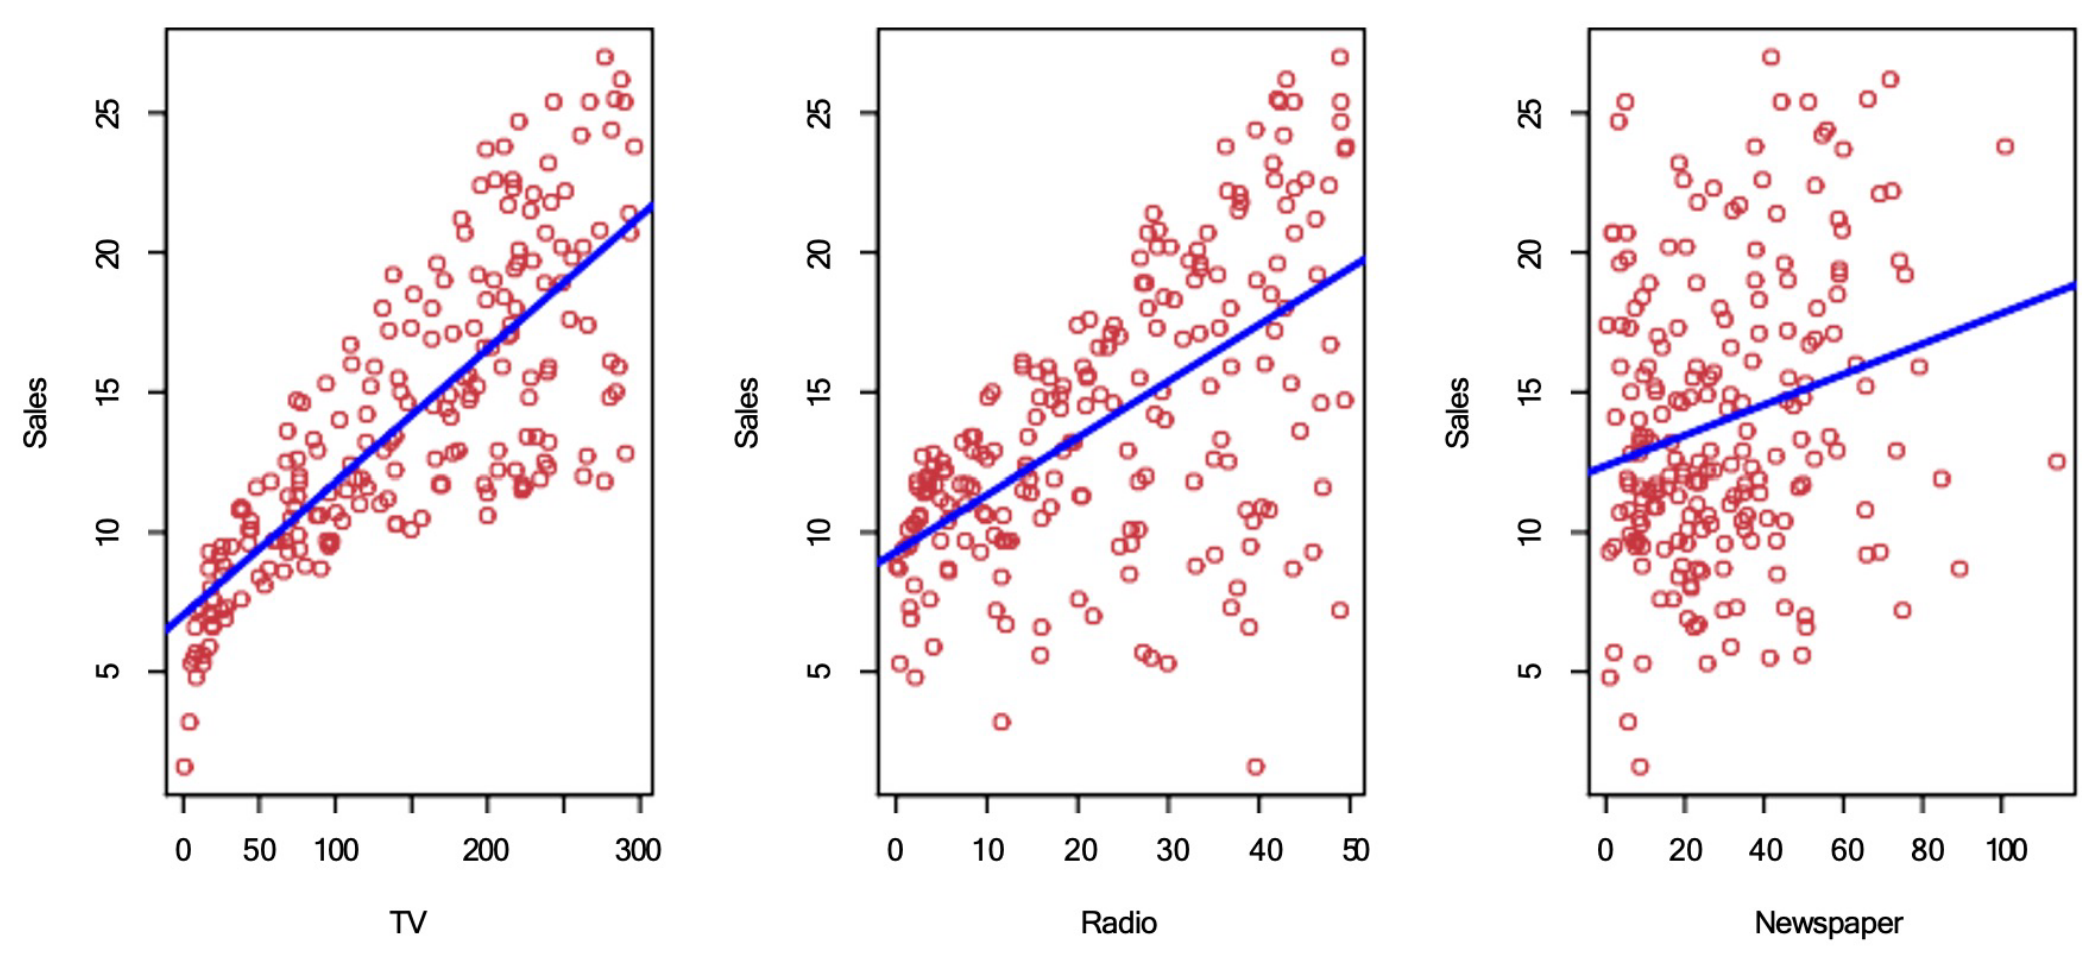
\includegraphics[width=0.8\textwidth]{images/multivariate-data-01}
\end{figure}

Here, the matrix $\mathbb X$ can be represented as

\begin{figure}[H]
	\centering
	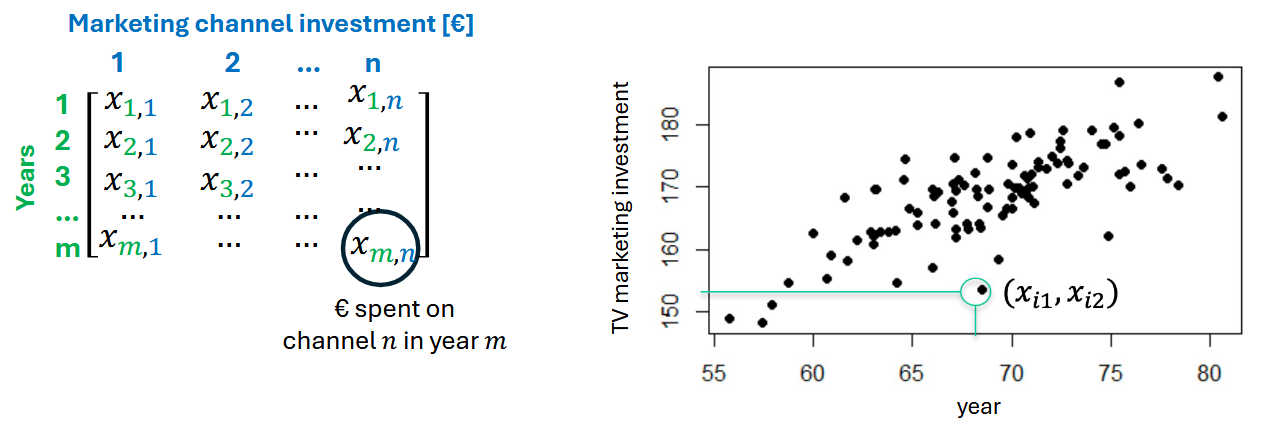
\includegraphics[width=0.9\textwidth]{images/multivariate-data-02}
\end{figure}

where the $i$-th row represents a set of coordinates in a multi-dimensional space.

\subsubsection{Supervised learning}

In the data, it is often possible to identify a specific target variable that we want to analyze or predict. This scenario is known as a \textbf{supervised learning} problem. In our example:

\begin{itemize}
	\item \textit{sales} is the \textbf{target} (or response) we want to predict, generally referred to as $y$;
	\item \textit{TV}, \textit{radio}, \textit{newspaper} are the \textbf{features} (or input, or predictors), named $x_1, x_2, x_3$.
\end{itemize}

The relationship between the features and the target is modelled mathematically as $y = f(X) + \varepsilon$, where $X = (x_1, x_2, x_3)$. If the target $Y$ is a continuous number, the task is defined as a \textbf{regression problem}, otherwise if $Y$ a categortical value, the task becomes a \textbf{calssification problem}.

The ultimate goal of finding a good function $f$ is twofold. First, it allows us to make accurate predictions of $Y$ at new, unseen points where $X = x$. Second, it helps us understand the underlying mechanics of the data: we can identify which comnponents of $X$ are crucial in explaining $Y$, and which are irrelevant, and how each feature impacts the target.

\subsubsection{Unsupervised learning}

Not all data, however, comes with a predefined target variable. \textbf{Unsupervised learning} operates on \textbf{unlabeled data}. Because there is no target $Y$ to predict, the algorithm's primary task is exploratory, analyzing the matrix $\mathbb X$ to discover inherent structures, hidden patterns, or relationships on its own. Conceptually, the model attempts to map the data back to itself, represented as $f(X) \approx X$.

\subsection{The prediction problem}

When building learning systems, the main task is making accurate predictions about unseen data. Consider the following example: \textit{what prediction should we make if we're asked to predict the height of the next student entering the classroom, to minimize the squared prediction error?}

The \textbf{Mean Squared Error (MSE)} measures the average of the squares of out errors, represented mathematically as
\begin{equation*}
	\frac 1 n \sum_{i = 1}^n \left( \hat y_i - y_i \right)^2
\end{equation*}
where $\hat y_i$ is the predicted target variable, $y_i$ is the true target variable, and $n$ is the number of samples.

If we knew all the heights of all students in the full population, the optimal prediction would simply be the population mean, denoted as $\mu$.

Even in this ideal scenario, our prediction error would not be zero, it would be equivalent to the variance of the through height $Y$ of the next student entering the classroom:
\begin{equation*}
	E_Y \left[ \left( Y - \mu \right)^2 \right]
	=
	Var(Y) = \sigma^2
\end{equation*}
this is known are \textbf{irreducible error}, we can't do better than this with any other prediction.

In reality, we don't even have access to the full population or the exact value of $\mu$. To understand how our model behaves under uncertainty, we can imagine a though experiment: drawing a sample of 10 students from the population repeatedly. Each time we resample, we create a new "parallel universe". In each universe, we collect a new sample of heights: $\bm{Y} = (Y_1, Y_2, \dots, Y_{10})$, and we use this sample to make a prediction, e.g., the sample mean $\bar{\bm{Y}}$. By observing the distribution of these predictions across all "parallel universes", we generate a sampling distribution.

By analyzing the average MSE of these predictions, we can decompose the error to understand its origins. The average MSE of these predictions is:
$$
	Average MSE = E_{Y, \bm Y}\left[\left( \hat Y - Y \right)^2 \right]
$$
There are two key sources beyond the irreducible error: \textbf{bias} and \textbf{variance}.

\subsubsection{Bias and Variance}

\textbf{Bias} is the difference between the mean of our sampling distribution and the actual population mean $\mu$, defined as
$$
	Bias = E_{\bm Y}[\bar Y] - \mu
$$
If our model's predictions are systematically too high or too low (on average across all "parallel universes'), the model exhibits bias.

The \textbf{variance} measures how much our prediction (i.e., the sample mean) fluctuates from one universe to the next, defined as
$$
	Var_{\bm Y}(\bar Y) = E_{\bm Y}\left[ \left( \bar Y - E_{\bm Y}[\bar Y] \right)^2 \right]
$$
If our predictions are highly sensitive to the specifice training sample drawn, the model has high variance.

\subsubsection{Bias-variance trade-off}

Suppose we fit a model $\hat f(X)$ to some training data and evaluate it on a new test observation $(x_0, y_0)$. If the true model is $Y = f(X) + \epsilon$ (with $f(X) = E(Y | X = x)$), then the expected prediction error can be explicitly broken down into three components:
$$
	E[y_0 - \hat f(x_0)]^2
	=
	\underbrace{Var[\hat f(x_0)]}_{\text{variance}}
	+
	\underbrace{Bias[\hat f(x_0)]^2}_{\text{bias}}
	+
	\underbrace{Var[\varepsilon]}_{\text{noise}}
$$
where $Bias[\hat f(x_0)] = E[\hat f(x_0)] - f(x_0)$.
\begin{itemize}
	\item \textbf{Variance}: captures how much the model changes if you train it on a different training set. High variance indicates the model is \textit{over-specialized} or \textit{over-fitting} to its specific dataset.
    \item \textbf{Bias}: what is the inherent error that you obtain from your model, even with infinite training data. This is due to the model being \textit{biased} to a particular kind of solution.
    \item \textbf{Noise}: measures ambiguity due to the data distribution and feature representation. You can never beat this, it is an aspect of the data.
\end{itemize}
